%************************************************
\chapter{Progettazione}\label{ch:progettazione}
%************************************************
Il seguente capitolo descrive le scelte progettuali che sono state effettuate, ovvero viene presentata l'architettura del sistema attraverso diagrammi delle classi e vengono illustrate le interazioni dell'utente col sistema attraverso i diagrammi di attività.

\section{Sencha Touch 2}
JavaScript, il linguaggio con cui è stato scritto il framework Sencha Touch, è un linguaggio di scripting prototype-based e multi-paradigma, supporta infatti sia la programmazione imperativa e object-oriented che quella funzionale.

Tali caratteristiche lo rendono un linguaggio molto flessibile che permette di risolvere lo stesso problema in molti modi e con differenti tecniche; purtroppo la mancanza di struttura nel linguaggio porta il grande svantaggio dell'imprevedibilità.

Inoltre, ogni chiamata a funzione che viene effettuata è asincrona, il che rende ancora meno semplice addomesticare il linguaggio ai propri scopi.

I progettisti di Sencha Touch hanno quindi cercato di dare una struttura solida al framework creando una gerarchia di oggetti e modellando attorno ad essi un'architettura \ac{MVC}.

Il risultato ottenuto è che ogni applicazione che si intende sviluppare con tale framework deve seguire correttamente tale pattern per riuscire a sfruttare appieno il sistema di classi messo a punto dai progettisti.

\begin{figure}[htb]
\centering
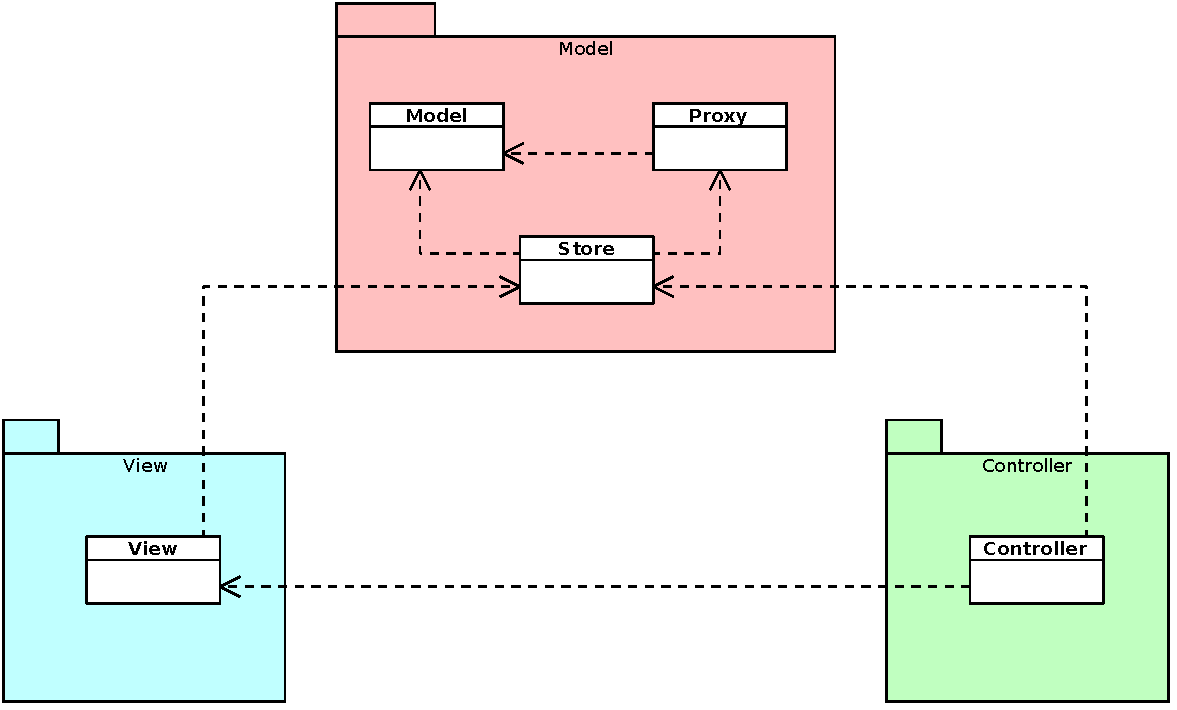
\includegraphics[scale=0.5]{gfx/class/Sencha_Touch_2.pdf}
\caption{Architettura generale Sencha Touch 2}
\label{fig:architettura Sencha}
\end{figure}

Il diagramma in figura \ref{fig:architettura Sencha} rappresenta l'architettura generale che ogni applicazione deve avere, ciò è riflesso anche nella struttura di cartelle e nei nomi dei file; essa si basa sul pattern architetturale \ac{MVC} il quale è composto da 3 package che svolgono funzioni diverse:
\begin{description}
\item[model:] rappresenta il modello dei dati su cui si basa l'applicazione; ogni oggetto model viene gestito da uno \emph{store} che si occupa di leggere e scrivere i dati mediante un \emph{proxy};
\item[view:] rappresenta tutti gli oggetti che servono a visualizzare le informazioni all'utente e si riflette dunque sull'interfaccia grafica;
\item[controller:] rappresenta il gestore della logica dell'applicazione; esegue il collegamento tra l'azione che l'utente desidera svolgere e i dati effettivi sul quale l'azione deve essere eseguita.
\end{description}

\section{Descrizione architettura}
\subsection{MyNotes}

\subsection{SensorDevice}


\section{Diagrammi di attività}